\chapter{Material and Methods}
\section{Invitrodb}
The most recent release of the Toxicity Forecaster database, referred to as \href{https://cfpub.epa.gov/si/si_public_record_Report.cfm?dirEntryId=355484&Lab=CCTE}{ToxCast's invitroDBv3.5}, represents an extensive collection of high-throughput screening (HTS) targeted bioactivity data. This database encompasses information on a total of 9541 compounds, selectively screened across 2205 assay endpoints. The establishment of this resource owes its origins to the collaborative endeavors of two prominent institutions: the United States Environmental Protection Agency (\href{https://www.epa.gov/chemical-research/exploring-toxcast-data}{EPA}) through its ToxCast program and the National Institutes of Health (\href{https://ntp.niehs.nih.gov/whatwestudy/tox21}{NIH}) via the Tox21 initiative. Incorporating data collected from diverse research laboratories, this relational database is openly accessible to the public and can be downloaded directly from the official ToxCast website.




\subsection{Presence matrix}
Consider a collection of $m$ assay endpoints, denoted by $A = \{a_1, a_2, \dots, a_m\}$ and a set of $n$ compounds represented as $C = \{c_1, c_2, \dots, c_n\}$.
To facilitate data comprehension, we introduce a \emph{presence matrix} $P \in {\{0, 1\}}^{m \times n}$. Rows, indexed by $i$, represent assay endpoints $a_i$, while columns, indexed by $j$, denote presence (1) or absence (0) of compound $c_j$ in those endpoints. Matrix $P$ is sparse due to the selective testing of compounds across different assay endpoints. A compound is considered present in an assay endpoint if it has undergone testing and a corresponding concentration-response series is available.
See Figure~\ref{fig:presence_matrix_all} for a visual of the \emph{presence matrix} $P$ covering all assay endpoints and compounds in \textit{invitroDBv3.5}. 

\begin{figure}[h]  % Placement options: h (here), t (top), b (bottom), p (page)
    \centering
    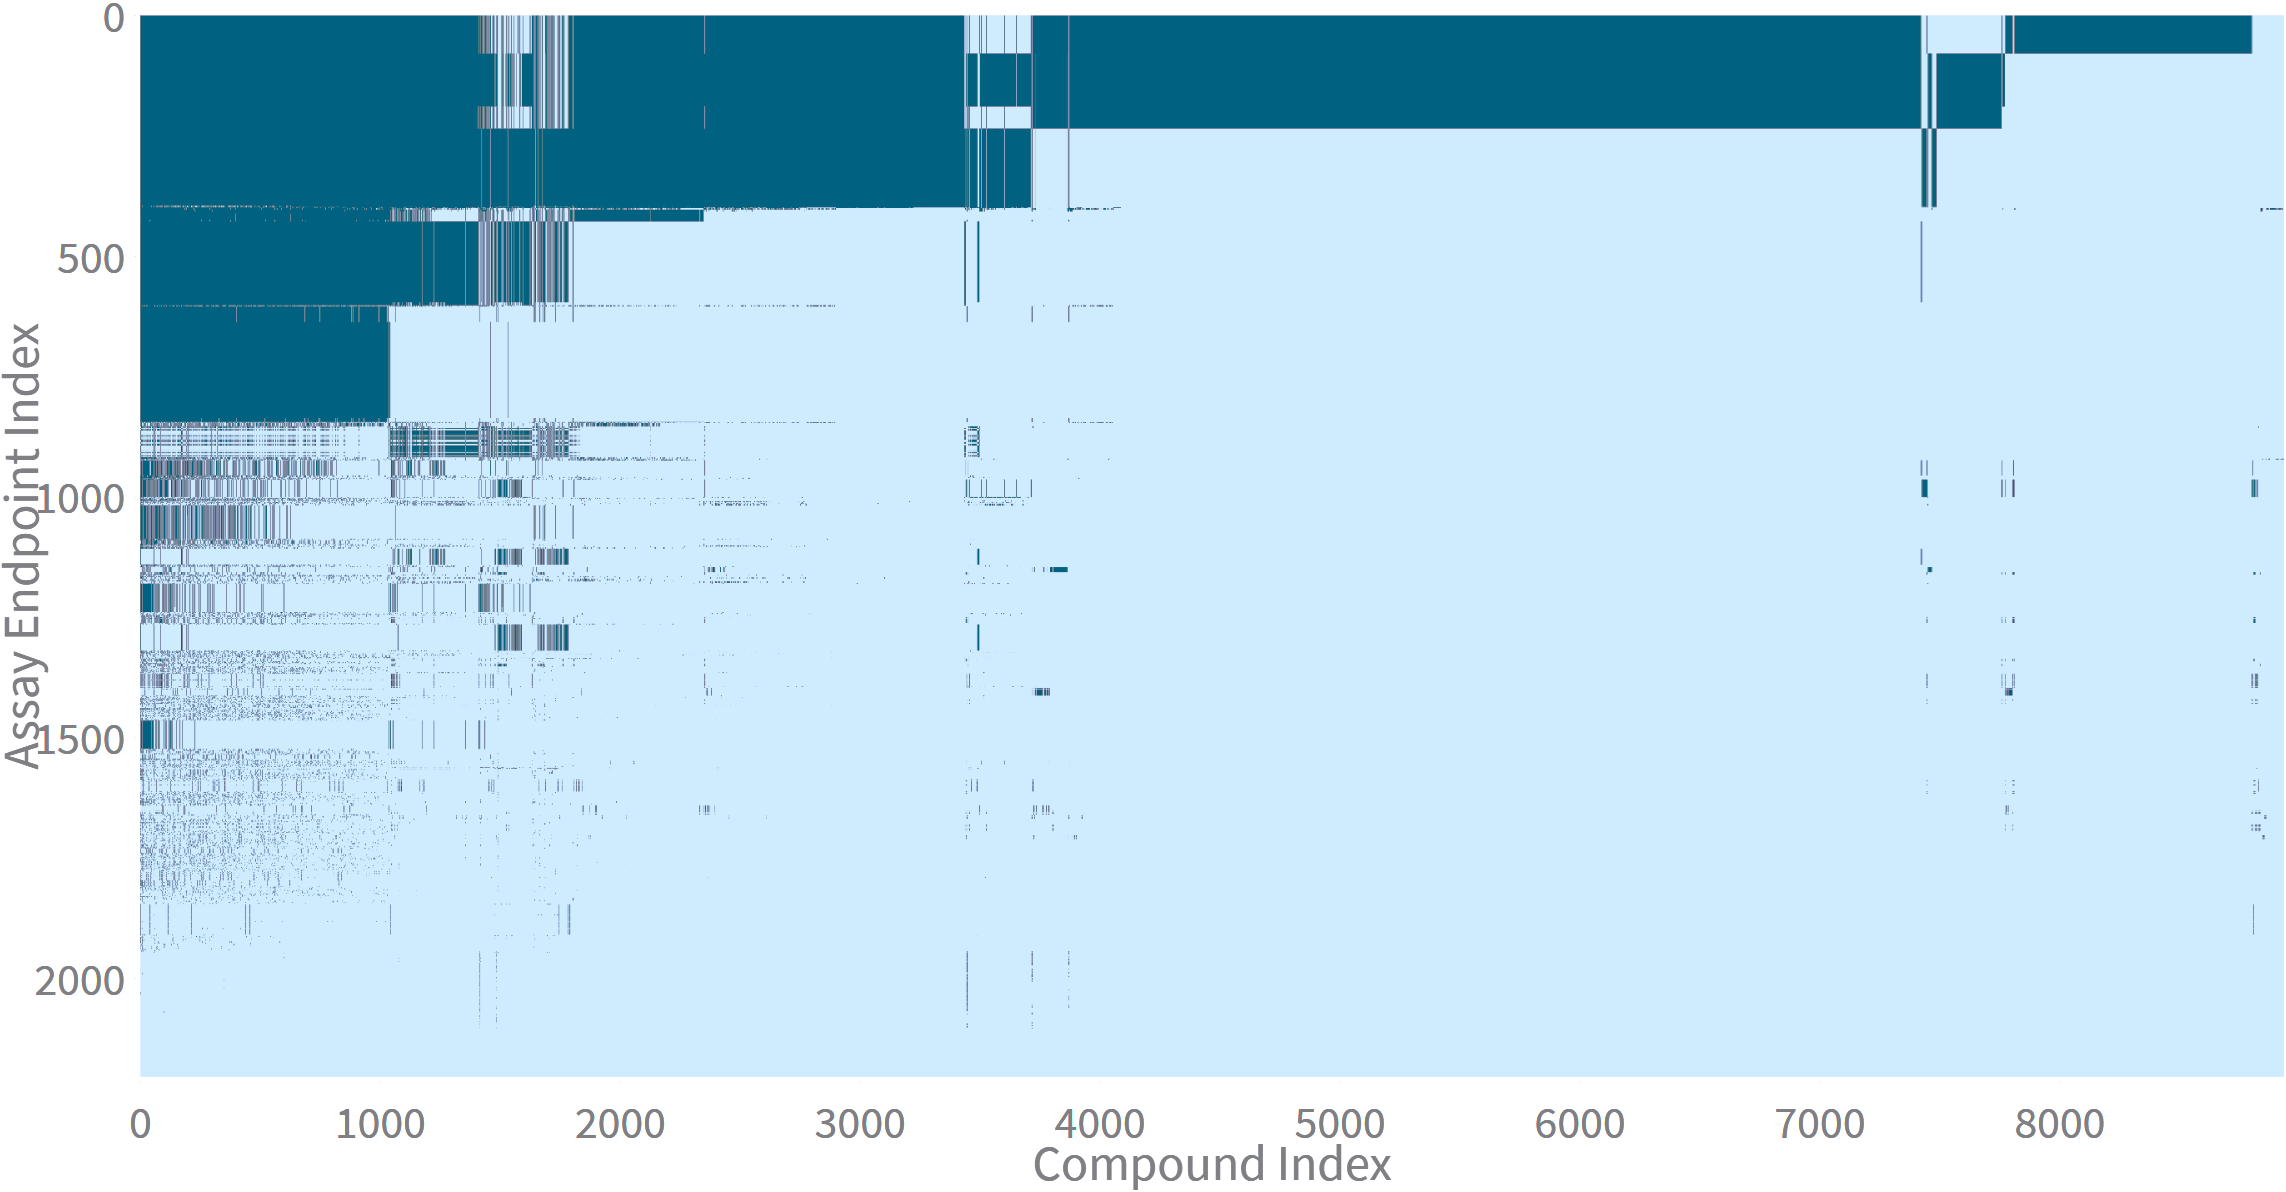
\includegraphics[width=1.0\textwidth]{figures/presence_matrix_all.png}  
    \caption{The \emph{presence matrix} $P$ covering all assay endpoints and compounds available in \textit{invitroDBv3.5} with $m = \num{2205}$ assay endpoints and $n = \num{9541}$ compounds. The count, where $P_{ij} = 1$, indicates the availability of \num{3342377} concentration-response series for downstream analysis.}
~\label{fig:presence_matrix_all} 
\end{figure}


A \textit{concentration-response series} is represented as a set of $k$ concentration-response pairs: 
\[ S = \{(conc_1, resp_1), (conc_2, resp_2), \dots, (conc_k, resp_k)\} \]
where $k$ $conc_i$ values are not necessarily unique. The quantity of concentration-response pairs exhibits considerable variability among different compounds tested across various assay endpoints.
In practice, concentrations are often subjected to multiple testing iterations, resulting in the formation of $n_{conc}$ distinct concentration groups. Within each concentration group, the number of replicates is indicated by $n_{rep}$.
Concentrations are transformed to the logarithmic scale using the unit $\mu M$ (micromolar), while the responses are normalized to either fold-induction or percent-of-control units.
Figure~\ref{fig:concentration_response_series} showcases a concentration-response series for a compound tested within a single assay endpoint.

\begin{figure}[htbp]  % Placement options: h (here), t (top), b (bottom), p (page)
    \centering
    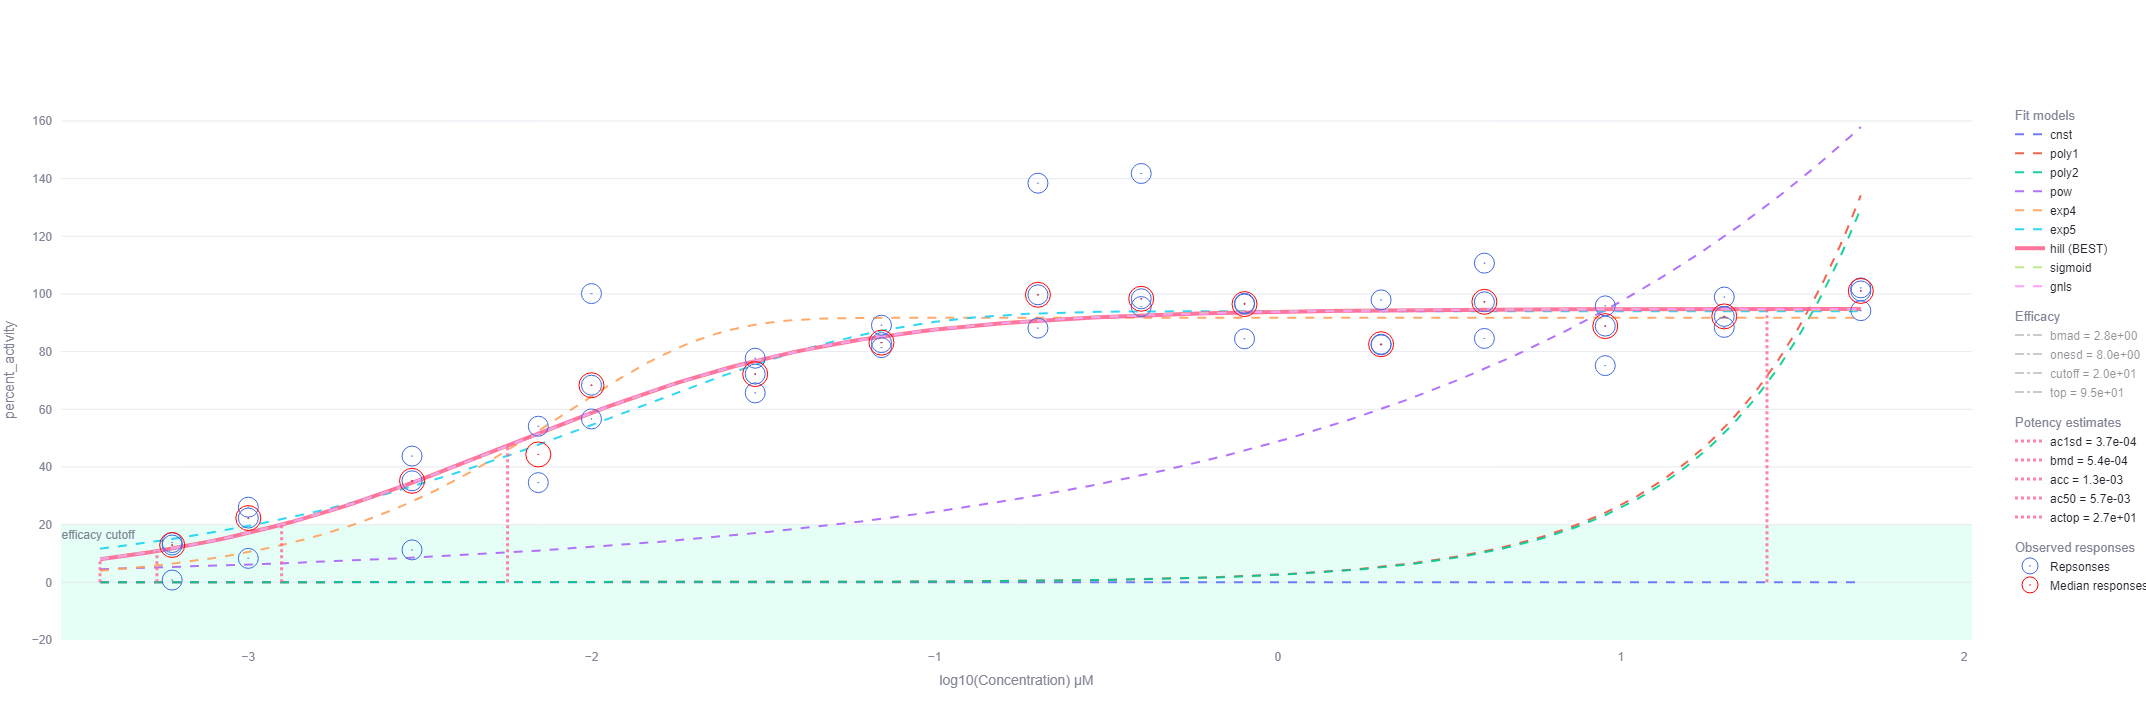
\includegraphics[width=1.0\textwidth]{figures/concentration_response_series_2.png}  
    \caption{A concentration-response series for the compound \textit{Estropipate} in the assay endpoint \textit{TOX21\_ERa\_LUC\_VM7\_Agonist}. The series has a total of $k = 45$ concentration-response pairs and is composed of $n_{conc} = 15$ concentration groups, each with $n_{rep} = 3$ replicates.}
~\label{fig:concentration_response_series} 
\end{figure}



\section{Pytcpl}
We introduce \href{https://github.com/rbBosshard/pytcpl}{pytcpl}, a streamlined Python package inspired by the R package \href{https://github.com/USEPA/CompTox-ToxCast-tcpl}{tcpl}, designed for processing high-throughput screening data. The package primarily focuses on providing essential features such as concentration-response curve fitting and allows for continuous hit-calling for compound bioactivity across diverse assay endpoints, akin to \href{https://github.com/USEPA/CompTox-ToxCast-tcplFit2}{tcplfit2}. \href{https://cfpub.epa.gov/si/si_public_record_Report.cfm?dirEntryId=355484&Lab=CCTE}{Invitrodb version 3.5 release} can optionally serve as backend database if desired. The package optimizes data storage and provides compressed raw data and metadata from \emph{invitroDB} in Parquet files. This efficient strategy reduces storage needs, resulting in just 4 GB within the repository—compared to the original 80 GB database. This obviates the need for a cumbersome, large-scale database installation, rendering downstream analysis more accessible and efficient. Our package is crafted to accomodate cusomizable processing steps and facilitate interactive data visualization with \href{https://pytcpl.streamlit.app/}{curve surfer} and empowers Python-oriented researchers to seamlessly engage in data analysis and exploration.
\subsection{Preprocessing}
First, all datapoints are collected from the database and assigned to the concentration response-series belonging to the respective ocompoud in the corresponding assay endpoint. The data is then filtered by the following criteria:

Data collection
Compute efficacy cutoff
Meet onditions for curve fitting
\subsection{Curve Fitting}
Introduce all candidate fit models
\subsection{Hit Calling}
Akaike criterion, 3 probabilities 
\subsection{Curve Surfer}
Data visualization, overview of what is possible with the tool. Filter by assay endpoint, compound, etc.


\section{Machine Learning Pipeline}
\subsection{Preprocessing}
Subselecting the columns from the output tables generated by pytcpl: DTXSID identifier and continuous hitcall value. The feature inputs to the machine learning model is a molecular structure represented as fingerprint generated from a SMILES string uniquely determined by the compounds DTXSID identifier. The SMILES string is a linear representation of a compound's molecular structure. The SMILES string is converted to a molecular graph, which is then converted to a feature vector. The feature vector is then used to train a machine learning model. The machine learning model is then used to predict the hitcall value for a given compound. The machine learning pipeline is illustrated in Figure~\ref{fig:ml_pipeline}. 


\subsection{Binary Classification}
The goal is to predict whether a compound is active or inactive for a given assay endpoint. We can formulate this as a binary classification problem, where the input is the compound's molecular structure fingerprint and the output is the hitcall value binarized by some decision threshold. The hitcall value is rendered to a binary variable, where 1 indicates that the compound is active and 0 indicates that the compound is inactive.
\subsection{Regression}
\subsection{Massbank Validation}
